\documentclass[a4paper,14pt]{extarticle}

\usepackage[top=2.5cm, bottom=2.5cm, left=2.5cm, right=2.5cm]{geometry}
\usepackage[utf8]{inputenc}
\usepackage[russian]{babel}
\usepackage{graphicx}
\usepackage{caption}
\usepackage{subcaption}
\usepackage{chngcntr}
\usepackage{amsmath}
\usepackage{amsfonts}
\usepackage{pgfplots}
\usepackage{pgfplotstable}
\usepgfplotslibrary{fillbetween}
\usepackage{float}
\usepackage{lipsum}% http://ctan.org/pkg/lipsum
\usepackage{multicol}% http://ctan.org/pkg/multicol
\usepackage{hhline}
\usepackage{tabularx}
\usepackage{tikz,xcolor}
\usepackage{tkz-graph}
\usepackage{float}
\usepackage{mathtools}
\usepackage{todonotes}
\usepackage{listings}
\usepackage[makeroom]{cancel}

\usetikzlibrary{arrows, petri, topaths}

\counterwithin{figure}{section}
\counterwithin{equation}{section}
\counterwithin{table}{section}

\DeclareMathOperator*{\argmin}{arg\,min}
\DeclareMathOperator*{\argmax}{arg\,max}
\DeclareMathOperator{\sinc}{sinc}

\definecolor{mygreen}{RGB}{28,172,0} % color values Red, Green, Blue
\definecolor{mylilas}{RGB}{170,55,241}

\lstset{language=Matlab,%
  %  basicstyle=\color{red},
    breaklines=true,%
    morekeywords={matlab2tikz,ylim,xlim,square,ones,double},
    keywordstyle=\color{blue},%
    morekeywords=[2]{1}, keywordstyle=[2]{\color{black}},
    identifierstyle=\color{black},%
    stringstyle=\color{mylilas},
    commentstyle=\color{mygreen},%
    showstringspaces=false,%without this there will be a symbol in the places where there is a space
    numbers=left,%
    numberstyle={ \color{black}},% size of the numbers
    numbersep=15pt, % this defines how far the numbers are from the text
    emph=[1]{for,end,break,switch,case,otherwise},emphstyle=[1]\color{red}, %some words to emphasise
    %emph=[2]{word1,word2}, emphstyle=[2]{style},    
}


\begin{document}
\begin{titlepage}
\centering 
{\bfseries Санкт-Петербургский Политехнический Университет} \\
Институт компьютерных наук и технологий \\
Кафедра компьютерных систем и программных технологий \\
\vspace{5cm}
{\centering \textbf{Отчёт по лабораторной работе №1} \\ 
\vspace{0.15cm}
\textbf{Дисциплина}: Телекоммуникационные технологии \\
\vspace{0.15cm}
\textbf{Тема}: Сигналы телекоммуникационных систем} \\
\vspace{4cm}
\hfill {\bfseries Работу выполнил студент}  \\
\hfill гр. 33501/4 Леженин Ю.И. \\
\hfill {\bfseries Преподаватель}  \\
\hfill Богач Н.В.
\vfill
Санкт-Петербург \\
{\large \today\par}
\end{titlepage}

\section{Цель работы.}

Познакомиться со средствами генерации и визуализации простых сигналов.

\section{Постановка задачи.} 

В командном окне MATLAB и в среде Simulink
промоделировать синусоидальный и прямоугольный сигналы с раз-
личными параметрами. Получить их спектры. Вывести на график.

\section{Ход работы.}

\subsection{Ряд и интеграл Фурье.}

Любая ограниченная, кусочно-непрервыная периодическая функция, имеющая конечное число экстремумов на протяжении периода, может быть представлена в виде ряда Фурье: 
\begin{equation*}
\varphi_p (t) = \sum_{k = -\infty}^{\infty} C_k e^{j 2 \pi k f_1 t} ,
\label{f1}
\end{equation*}
где $f_1 = 1 / T_1$; $T_1$ -- период функции $\varphi_p (t)$; $C_k$ - постоянные коэффициенты.

Коэффициенты могут быть найдены следующим образом:
\begin{equation*}
C_k = \frac{1}{T_1} \int_{t_0}^{t_0 + T_1} \varphi_p (t) e^{-j 2 \pi k f_1 t} dt.
\label{f2}
\end{equation*}
При этом значение выражения не зависит от $t_0$. Обычно берется $t_0 = 0$ или $t_0 = - T_1 / 2$.

Приведенные формулы можно записать в виде одного выражения:  
\begin{equation*}
\varphi_p (t) = \sum_{k = -\infty}^{\infty} \bigg[ \frac{1}{T_1} \int_{t_0}^{t_0 + T_1} \varphi_p (t) e^{-j 2 \pi k f_1 t} dt \bigg] e^{j 2 \pi k f_1 t}.
\label{f3}
\end{equation*}

%todo phase

Ряд Фурье справедлив для периодических сигналов, однако на его основе можно вывести соотношения и для непериодических сигналов. В этом случае период $T_1 \rightarrow \infty$, в связи с этим частота $f_1 \rightarrow 0$ и обозначается как $df$, $k f_1$ является текущим значением частоты $f$, а сумма меняется на интеграл. В результате получается выражение 
\begin{equation*}
\varphi_p (t) = \int_{-\infty}^{\infty} \bigg[ \int_{-\infty}^{\infty} \varphi_p (t) e^{-j 2 \pi f t} dt \bigg] e^{j 2 \pi f t} df.
\label{f4}
\end{equation*}
Это выражение называется интегралом Фурье и объединяет прямое преобразование Фурье
\begin{equation*}
\Phi (f) = \int_{-\infty}^{\infty} \varphi (t) e^{-j 2 \pi f t} dt
\end{equation*}
и обратное преобразование Фурье
\begin{equation*}
\varphi (t) = \int_{-\infty}^{\infty} \Phi (f) e^{j 2 \pi f t} dt.
\end{equation*}

Приведенные преобразования существуют только для функций с ограниченной энергией:
\begin{equation*}
\int_{-\infty}^{\infty} |\varphi (t)|^2 dt \neq \infty
\end{equation*}

И ряд, и интеграл могут быть названы преобразованием Фурье (ПФ), но обычно этим термином обозначается именно интеграл Фурье. Преобразование Фурье сигнала так же называется спектром сигнала.

\subsection{Свойства преобразования Фурье.}

Преобразование Фурье имеет ряд свойств:

\begin{enumerate}

\item Суммирование функций. \\ Преобразование Фурье -- линейное преобразование. Отсюда следует 
\begin{equation*}
\sum_{i=1}^n \alpha_i \varphi_i (t) \leftrightarrow  \sum_{i=1}^n \alpha_i \Phi_i (f).
\end{equation*}   
где $\alpha_i$ -- постоянный коэффициент.

\item Смещение функций. \\ При смещении функции на $t_0$ ее ПФ умножается на $e^{j 2 \pi f t_0}$:
\begin{equation*}
\varphi (t - t_0) \leftrightarrow e^{-j 2 \pi f t_0} \Phi (f).
\end{equation*}

\item Изменение масштаба аргумента функции.
При домножении аргумента функции $t$ на постоянный коэффициент $\alpha$, ПФ функции имеет вид $\frac{1}{|\alpha|} \Phi \big(\frac{f}{\alpha}\big)$:
\begin{equation*}
\varphi(\alpha t) \leftrightarrow \frac{1}{|\alpha|} \Phi \bigg(\frac{f}{\alpha}\bigg).
\end{equation*}

\item Перемножение функций.  ПФ произведения двух функции равно свертки ПФ этих функций:
%  \int_{-\infty}^{\infty} \Phi_1(f')\Phi_2(f-f') df'=
\begin{equation*}
\varphi_1 (t) \varphi_2 (t) \leftrightarrow \Phi_1(f) * \Phi_2(f). 
\end{equation*}

\item Свертывание функций. \\ ПФ свертки двух функций равно произведению ПФ этих функций:
\begin{equation*}
\varphi_1(t) * \varphi_2(t) \leftrightarrow  \Phi_1(f)  \Phi_2(f).
\end{equation*}

\item Дифференцирование функции. \\ При дифференцировании функции ее ПФ домножается на $j 2 \pi f$:
\begin{equation*}
\frac{d[\varphi(t)]}{dt} \leftrightarrow j 2 \pi f \Phi (f).
\end{equation*}

\item Интегрирование функции. \\ При интегрировании функции ее ПФ делится на $j 2 \pi f$:
\begin{equation*}
\int_{-\infty}^{t} \varphi(t') dt' \leftrightarrow \frac{1}{j 2 \pi f} \Phi (f).
\end{equation*}

\item Обратимость преобразования. \\ Преобразование обратимо с точность до знака аргумента. 
\begin{gather*}
\varphi(t) \leftarrow \Phi (f) \\ \Phi(t) \leftrightarrow \varphi (-f), ~ \Phi(-t) \leftrightarrow \varphi(f)
\end{gather*}

\end{enumerate}  


\subsection{Основные классы сигналов и их спектры.}

Обычно классификация сигнала выполняется по ряду основных признаков: конечность, периодичность и дискретность.

Сигнал конечной длительности имеет значение только внутри определенного интервала и вне его принимает значение 0. Такой сигнал можно представить как произведение сигнала бесконечной длительности и прямоугольной функции:
\begin{equation*}
x_f (t) = x(t) \cdot \Pi(t, T) = \begin{cases} x(t), t \in [-T/2, T/2] \\ 0, t \notin  [-T/2, T/2] \end{cases}.
\end{equation*}
При применении ПФ к данному виду сигналов происходит сверка образа сигнала и образа прямоугольной функции:
\begin{equation*}
\Phi_f(f) = \Phi(f) * \frac{sin(\pi f T)}{\pi f} = \Phi(f) * \sinc(\pi f).
\end{equation*}

Периодический сигнал обладает свойством $x_p(t) = x_p(t - k\,T)$, где $ k \in \mathbb{Z}$, а $T$ -- период. Такой сигнал можно представить как свертку одиночного сигнала длительностью $T$ и последовательности дельта импульсов:
\begin{equation*}
x_p(t) = x_{pT}(t) * \text{Ш}(t, T).
\end{equation*}
При применении ПФ выполняется умножение образа функции на последовательность дельта импульсов. Спектр периодического сигнала дискретно и соотносится с ПФ одиночного сигнала следующим образом:
\begin{equation*}
\Phi_p(f) = \Phi_{pT}(f) \cdot \text{Ш}(f, \frac{1}{T}).
\end{equation*}

Дискретный по времени сигнал обычно состоит из набора равноотстоящих по времени отсчетов отсчетов. Его можно представить как произведение непрерывного сигнала и последовательности дельта импульсов:
\begin{equation*}
x_d(t) = x(t) \cdot \text{Ш}(t, T_s).
\end{equation*}
При выполнении ПФ произойдет свертка образа функции и последовательности импульсов. Спектр дискретного сигнала периодическая функция с периодом $\frac{1}{T_s}$:
\begin{equation*}
\Phi_d(f) = \Phi(f) * \text{Ш}(f, \frac{1}{T_s}).
\end{equation*}

\subsection{Спектры некоторых простых сигналов.}

В ходе работы была выполнена генерация нескольких сигналов разного вида. Каждый из обрабатываемых сигналов содержит 512 отсчетов, столько же отсчетов используется для построения его спектра. Так как, сигналы конечные и дискретные, полученные спектры периодичны и имеют искажения обусловленные сверткой с функцией $\sinc(\pi f)$. На рисунках ниже преобразование приведено на интервале $[-T_s / 2, T_s/2]$, что соответствует одному периоду.  


Спектр гармонического сигнала представляет собой набор дискретных отсчетов на частоте, которая совпадает с частой гармоник в сигнале. Значение спектра в отсчетах зависит от амплитуды соответствующих гармоник. 

На рисунке \ref{sin_x} приведен гармонический сигнал, описываемый выражением $x(t) = \sin(2 \pi f_0 t) + 0.2 \, \cos(2 \pi f_1 t), ~ f_0 = 10\text{Гц}, ~ f_1 = 2\text{Гц}$. На рисунке \ref{sin_s} приведен амплитудный спектр $|\Phi(f)|$ данного сигнала.	Спектр симметричен относительно 0, положение пиков соответствует частотам гармоник, входящих в состав сигнала. 

\begin{figure}[H]
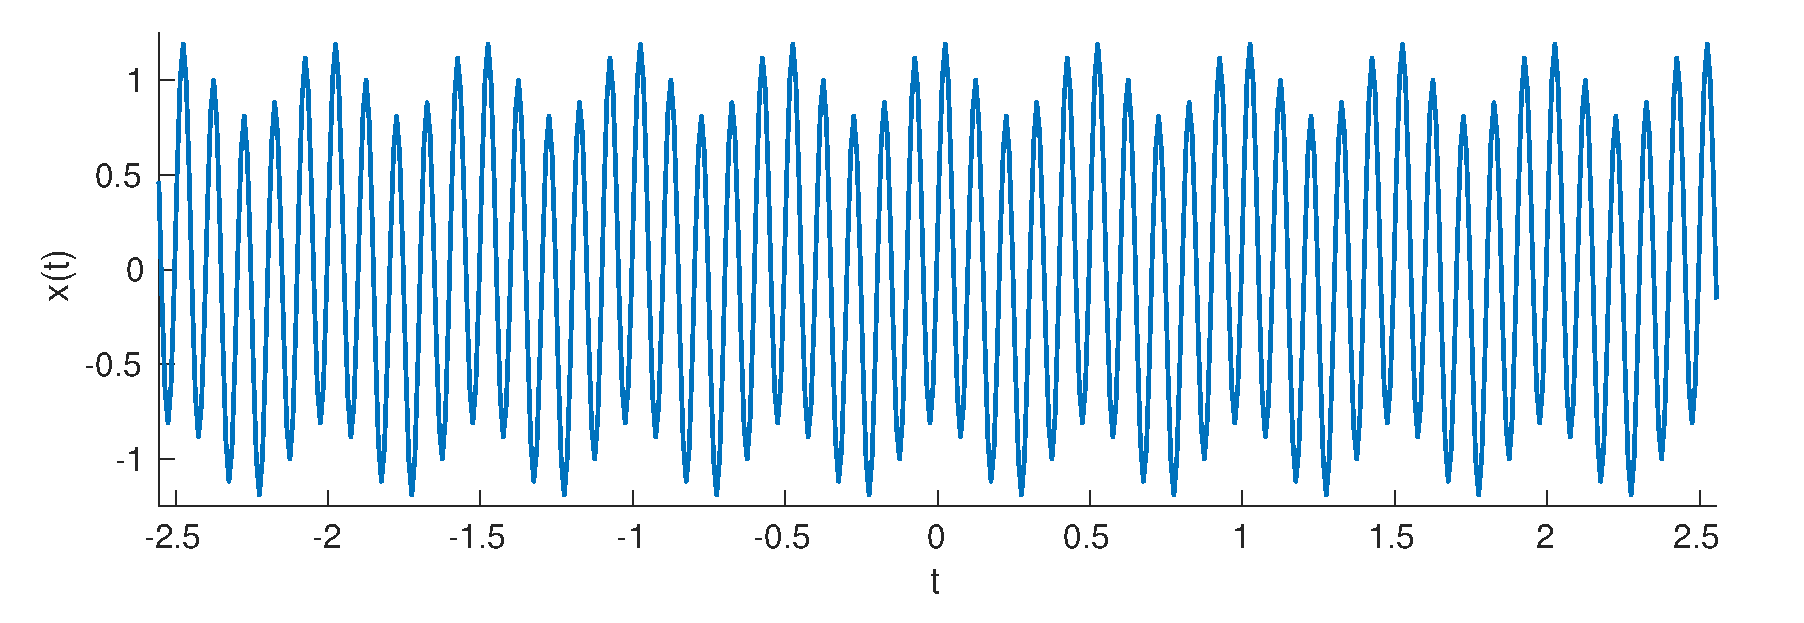
\includegraphics[width=1\textwidth]{sin_x.eps}
\caption{Гармонический сигнал.}
\label{sin_x}
\end{figure}

\begin{figure}[H]
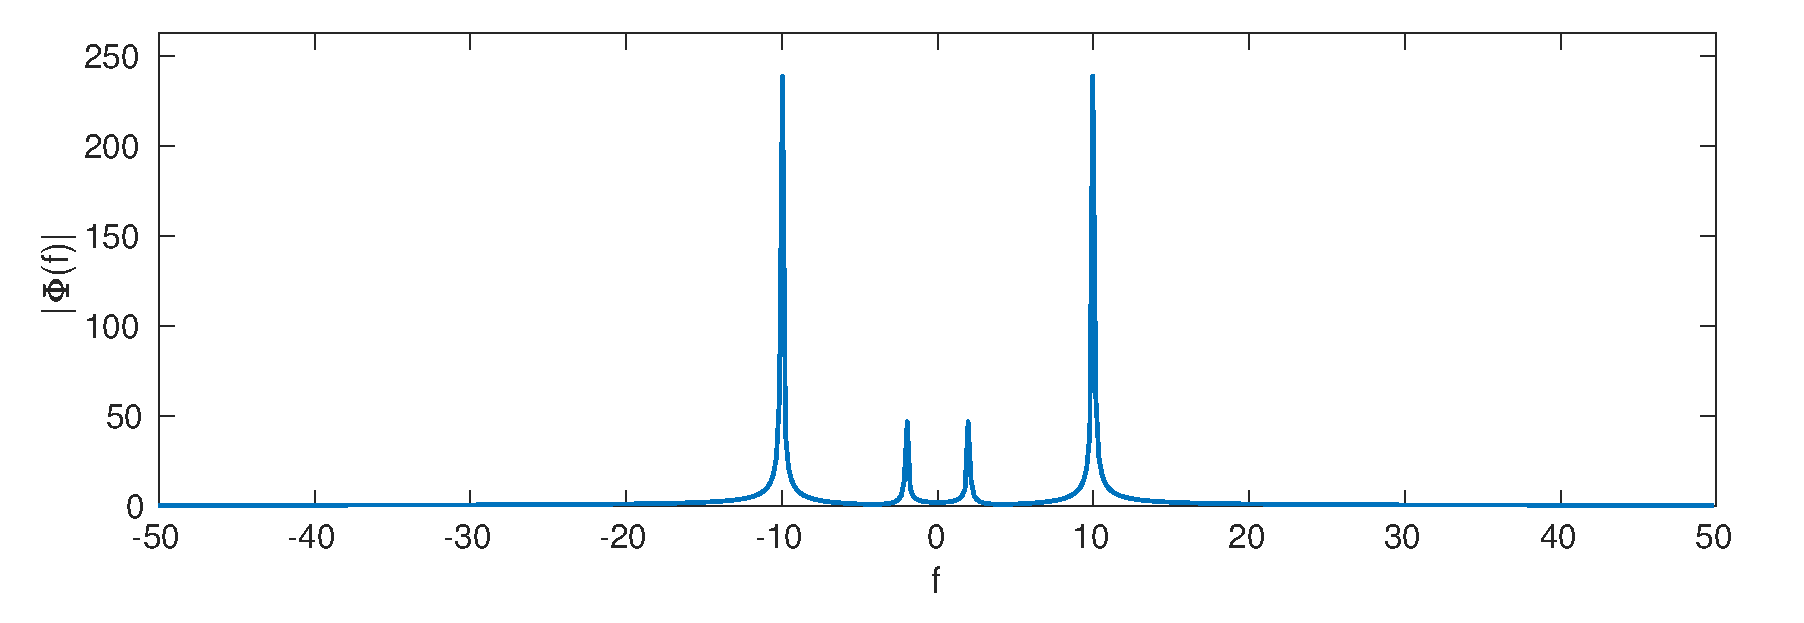
\includegraphics[width=1\textwidth]{sin_s.eps}
\caption{Амплитудный спектр гармонического сигнала.}
\label{sin_s}
\end{figure}

Спектром прямоугольного импульса длительностью $T_i$ является функция $\sinc(\pi f)=\frac{\sin(\pi f T_i)}{\pi f}$. При бесконечном повторении импульсов с периодом $T_0$ происходит дискретизация спектра, отсчеты находятся друг от друга на расстоянии $f_0 = 1/T_0$. 

Прямоугольный периодический сигнал с длительностью импульса $T_i = 0.1$ c и периодом $T = 0.2$ c приведен на рисунке \ref{sqr_x}, а его спектр -- на рисунке \ref{sqr_s}. Отсчеты в спектре находятся на расстоянии 10 Гц друг от друга, что соответствует $2f_0$. Это объясняется тем, что функция $\frac{\sin(\pi f T_i)}{\pi f}$ имеет корни в точках $f = k/T_i$, где $k$ -- целое число, а в данном случае $2\,T_i = T_0$. Получается, что в точках $f = k \cdot 2/T_0 =  2 \, k f_0$ спектр равен 0, а отсчеты находятся в точках $f = k f_0$. Таким образом, половина отсчетов равны нулю.

\begin{figure}[H]
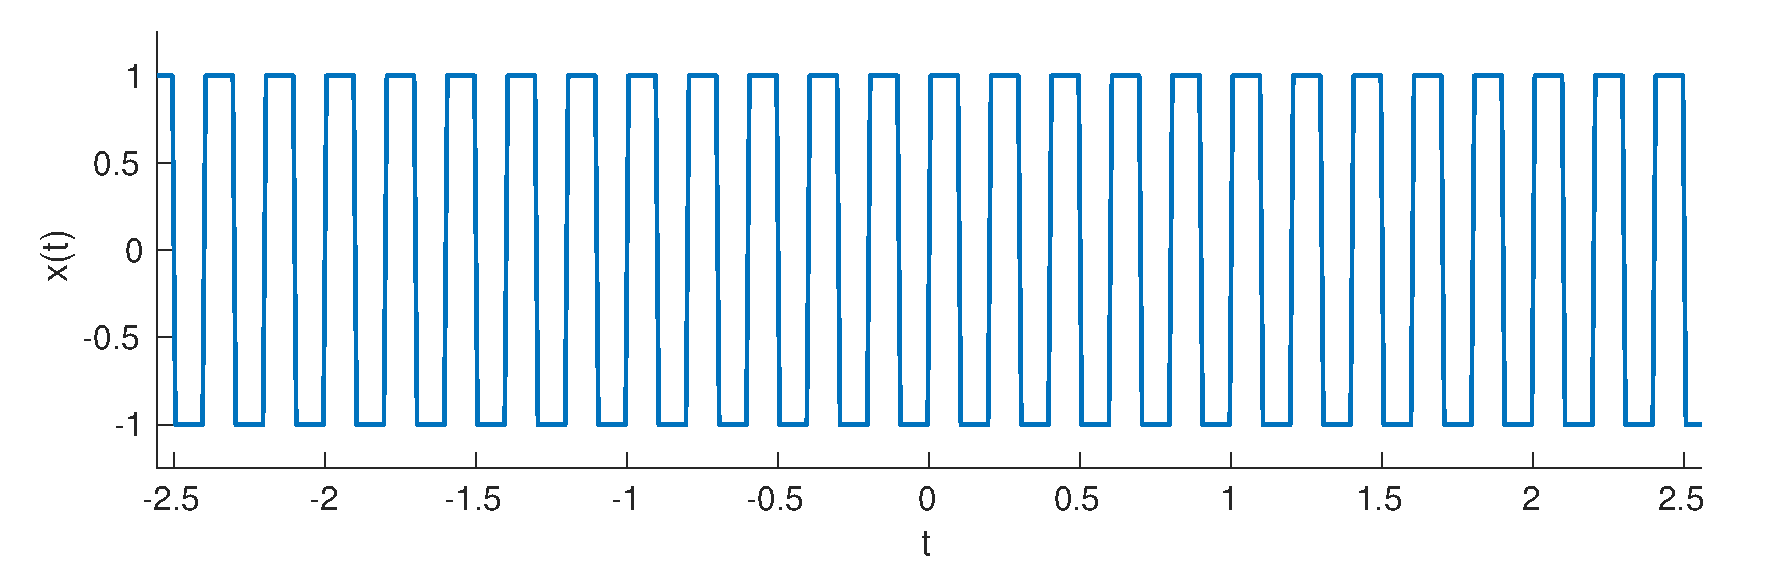
\includegraphics[width=1\textwidth]{sqr_x.eps}
\caption{Прямоугольный периодический сигнал.}
\label{sqr_x}
\end{figure}

\begin{figure}[H]
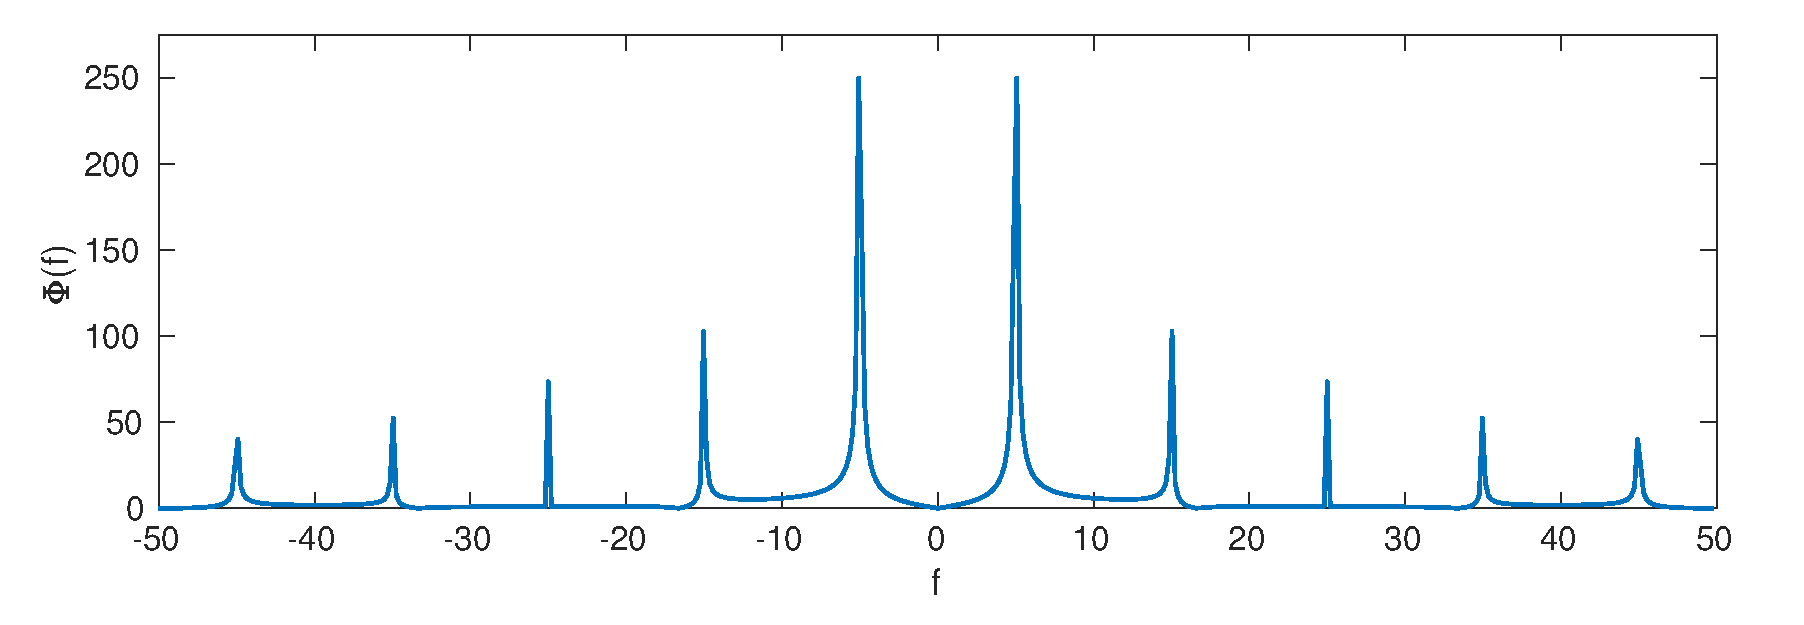
\includegraphics[width=1\textwidth]{sqr_s.eps}
\caption{Спектр прямоугольного периодического сигнала. }
\label{sqr_s}
\end{figure}

Треугольный импульс может быть представлен как свертка двух прямоугольных импульсов, таким образом спектр одиночного треугольного сигнала это функция $\sinc(\pi f)^2$.

Треугольный периодический сигнал с частотой $f_0 = 5~\text{Гц}$ приведен на рисунке \ref{trg_x}, его спектр приведен на рисунке \ref{trg_s}. Для данного случая справедливы те же рассуждения, что и для периодического прямоугольного сигнала.

\begin{figure}[H]
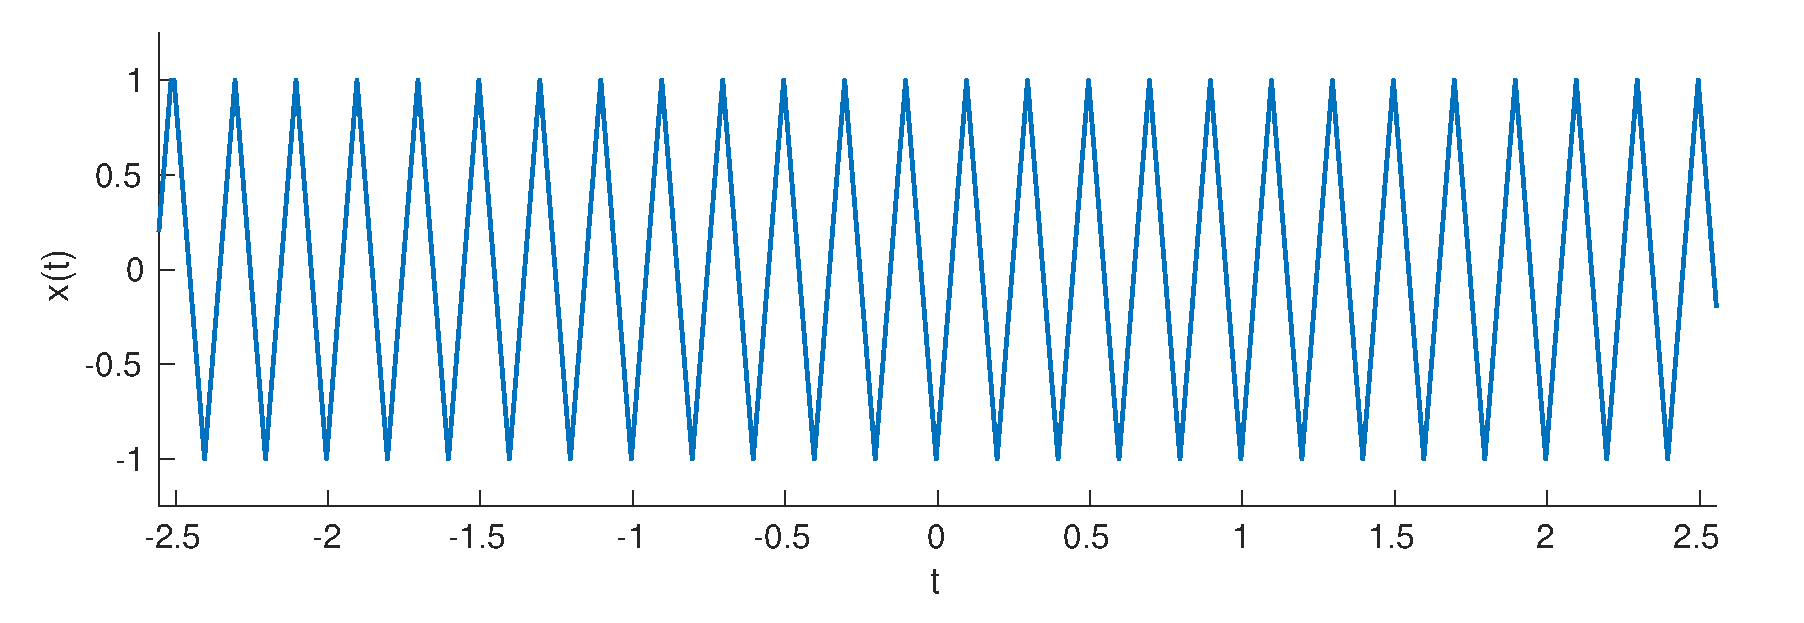
\includegraphics[width=1\textwidth]{trg_x.eps}
\caption{Треугольный периодический сигнал.}
\label{trg_x}
\end{figure}

\begin{figure}[H]
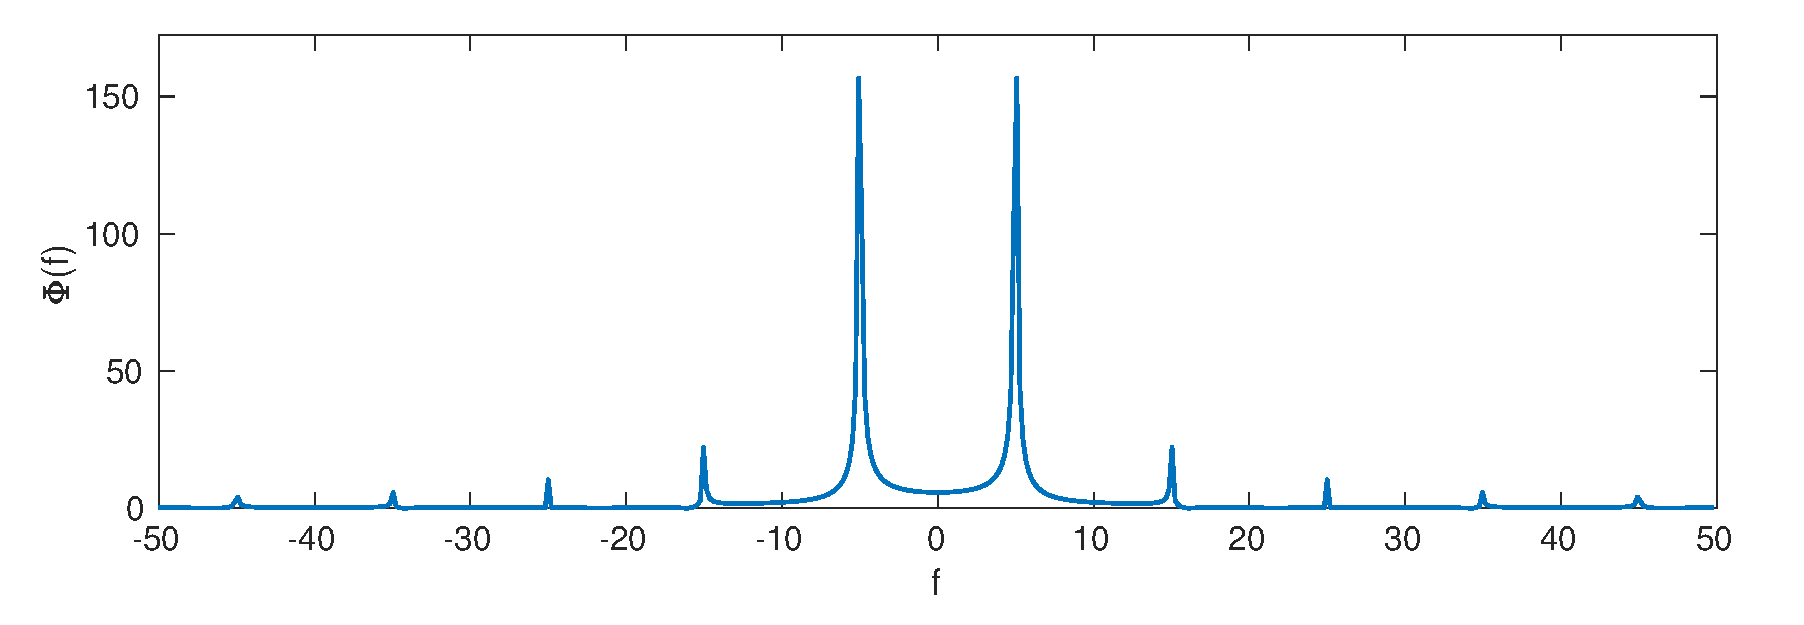
\includegraphics[width=1\textwidth]{trg_s.eps}
\caption{Спектр треугольного периодического сигнала.}
\label{trg_s}
\end{figure}


\section{Выводы.}

Преобразование Фурье позволяет представить сигнал в базисе гармонических колебаний разной частоты. Это значительно облегчает обработку и синтез сигналов.

Важнейшими свойствами ПФ являются теорема о свертывании сигналов и теорема о перемножении сигналов: произведение функций - это свертка их образов, свертка функций - это произведение их образов.

Спектр периодического сигнала дискретный, а дискретного - периодический. Если сигнал конечный, то при выполнении преобразования его образ сворачивается с функцией $\sinc(\pi f)$. 

\section{Приложение.}

\lstinputlisting[frame=single, caption=Программа для генерации приведенных сигналов и спектров.]{lab1_script.m}



\end{document}